
\section{Rückblick}

\begin{frame}
  {Rückblick: Syntax bisher}
  \pause
  \begin{itemize}[<+->]
    \item \alert{Phrasen} als Kopf und Abhängige
    \item Skepsis gegenüber "`Satzgliedern"'
      \Halbzeile
    \item Nebensätze als syntaktischer Basisfall
    \item unabhängige Sätze als Ergebnis von \alert{Umstellungen} (\textit{Bewegung})
    \item Sätze als kopflos
      \Halbzeile
    \item Funktion von unabhängigen Sätzen: \rot{nicht die \textit{Sprechaktfähigkeit}}
    \item Definition unabhängiger Sätze rein syntaktisch
      \Halbzeile
    \item Funktion von satzartigen Konstituenten\\
      (nicht Frage- und Befehlssätze):
      \begin{itemize}[<+->]
        \item \textit{Einschlussrelation} von Sachverhalten (Komplement-\slash Ergänzungssatz)
        \item rhetorische\slash pragmatische Relationen zwischen Sachverhalten\\
          (Adverbial-\slash Angabensatz)
        \item Kodierung zusätzlicher Sachverhalte über Objekte (Relativsatz)
      \end{itemize}
  \end{itemize}
\end{frame}


\begin{frame}
  {Übrigens: grammatische Mittel und Bildungssprache}
  \pause
  Aus \citet{Feilke2012}\\
  \Halbzeile
  \pause
  \centering
  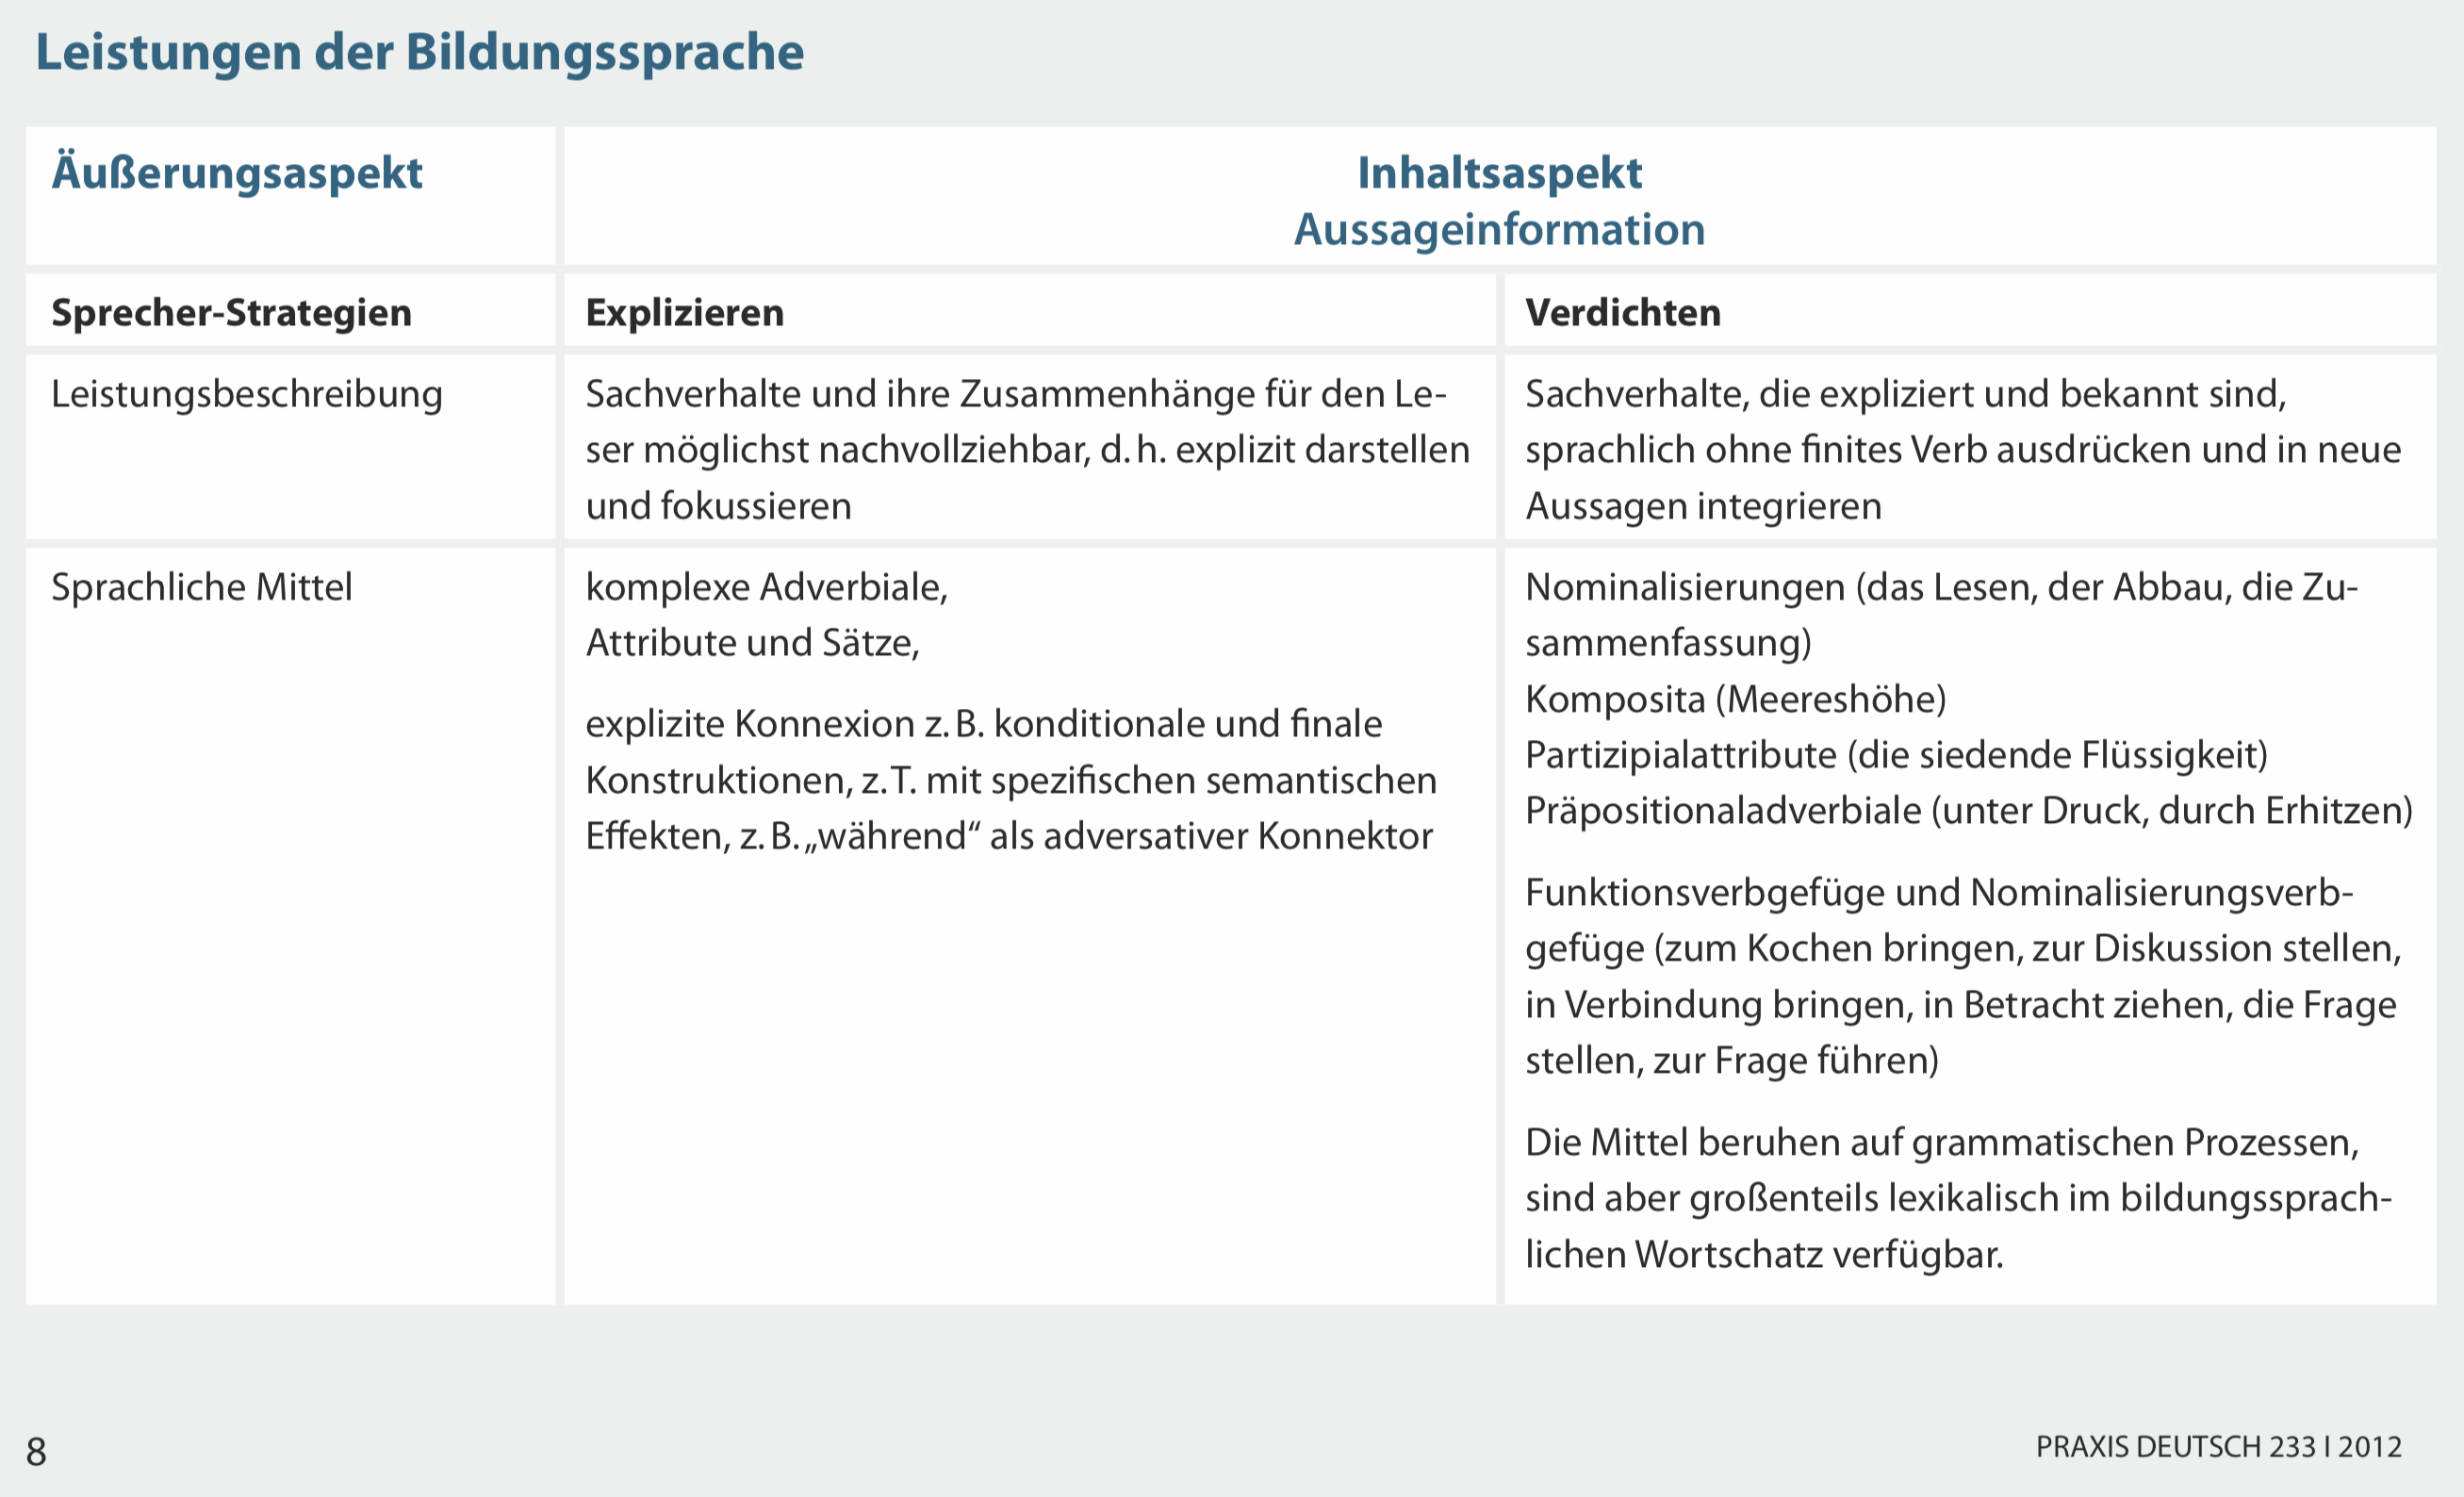
\includegraphics[width=0.9\textwidth]{\GRAPHPATH/feilke1}
\end{frame}


\begin{frame}
  {Übrigens: grammatische Mittel und Bildungssprache}
  \pause
  Aus \citet{Feilke2012}\\
  \Halbzeile
  \pause
  \centering
  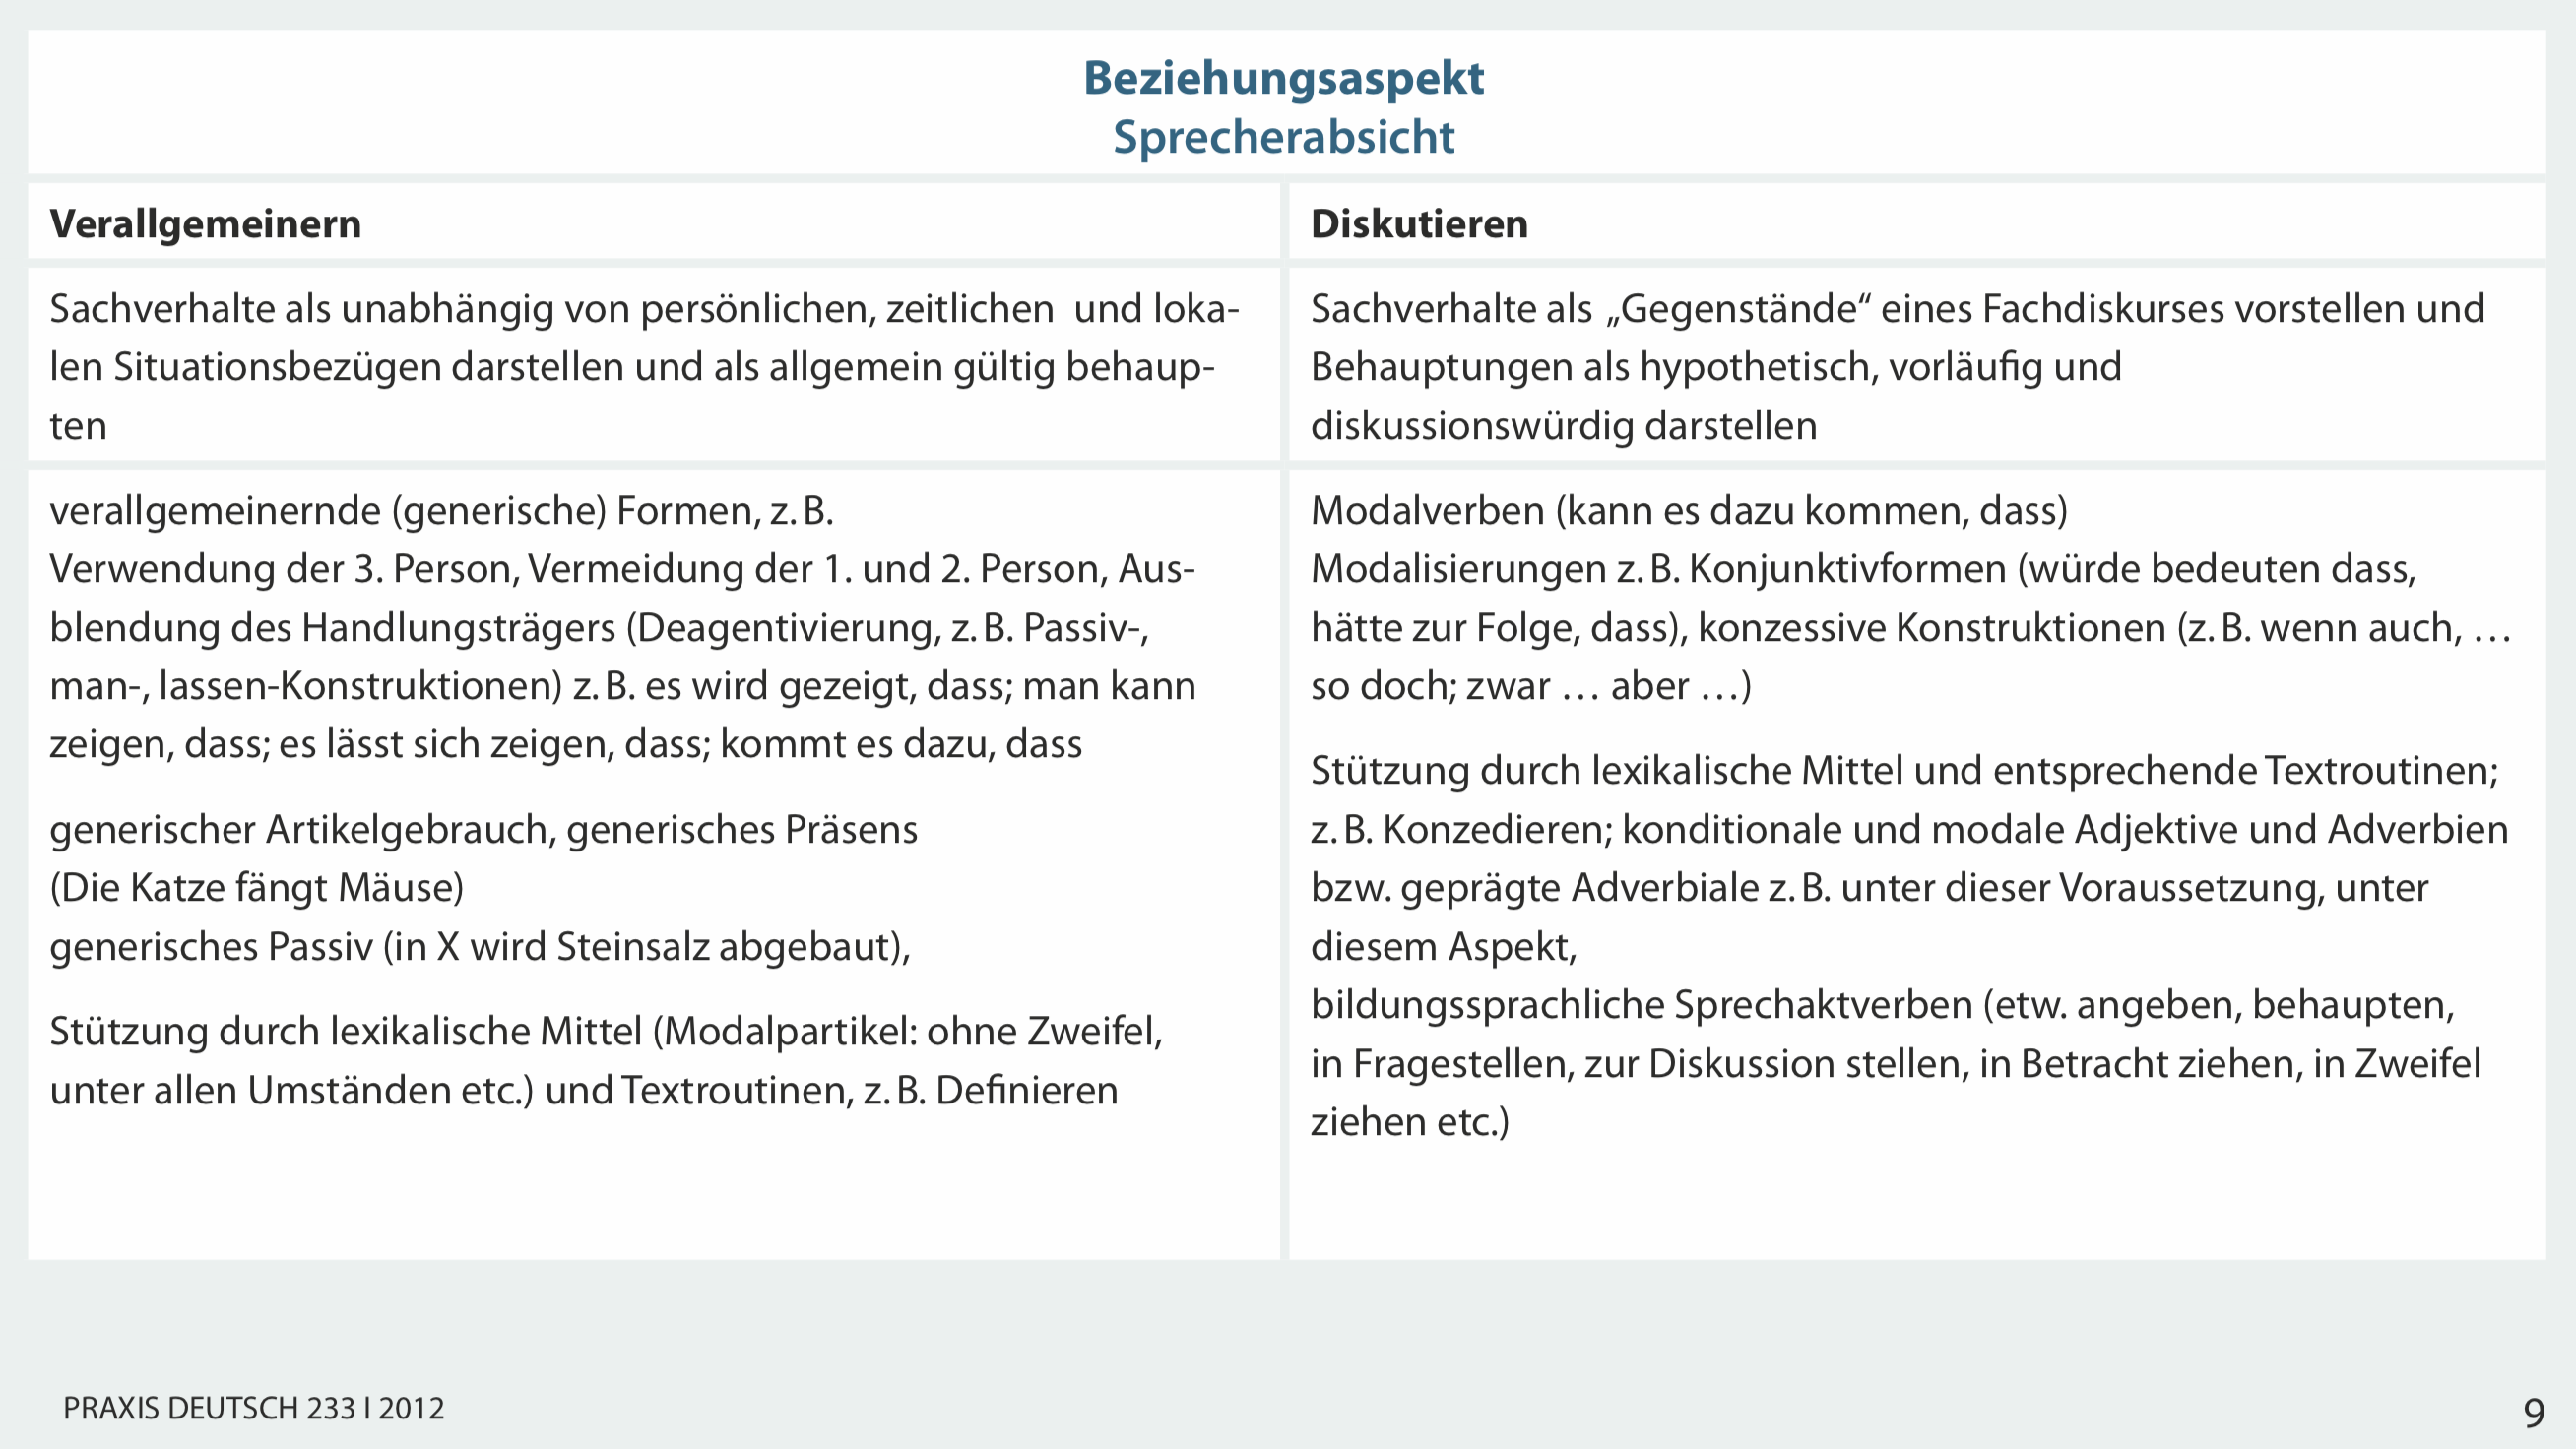
\includegraphics[width=0.9\textwidth]{\GRAPHPATH/feilke2}
\end{frame}


\section{Überblick}

\begin{frame}
  {Relationen und Prädikate}
  \pause
  \begin{itemize}[<+->]
    \item Verbsemantik und Valenz: semantische Rollen
      \Halbzeile
    \item Warum ist der Begriff \textit{Subjekt} überflüssig?
    \item Warum ist der Begriff \textit{Prädikat} problematisch?
    \item Wieviele Passive gibt es, und welche Verben sind passivierbar?
    \item Was sind direkte, indirekte und PP-Objekte?
    \item Und was sind Dativ- und PP-Angaben?
      \Halbzeile
    \item \alert{Valenzänderungen} und \alert{Valenzerweiterungen}
      \Halbzeile
    \item Gerade \alert{wegen} der Schwierigkeiten mit der Schulterminologie\\
      wird hier heute Wichtiges gelernt!
  \end{itemize}

\end{frame}

\begin{frame}
  {Relationen?}
  \pause
  \begin{itemize}[<+->]
    \item \alert{Kategorien}
      \begin{itemize}[<+->]
        \item Wortklasse?
        \item Numerus
        \item Tempus
        \item Komparationsstufe
        \item Kasus?
          \Halbzeile
        \item \alert{für die jeweilige Einheit definiert}
      \end{itemize}
      \Halbzeile
    \item \alert{Relationen}
      \begin{itemize}[<+->]
        \item Subjekt, Objekt (zum Verb)
        \item Ergänzung\slash Angabe (zu einem Wort)
        \item Prädikat (eines Satzes?)
        \item Attribut (zu einem Nomen)
          \Halbzeile
        \item \alert{zwischen Einheiten definiert}
        \item \alert{erfordern oft bestimmte Kategorien}
      \end{itemize}
  \end{itemize}
  \pause
  \Halbzeile
  \rot{Relationen helfen, syntaktische Strukturen zu dekodieren.}
\end{frame}

\section{Semantische Rollen}

\begin{frame}
  {Semantik-Grammatik-Schnittstelle}
  \pause
  \begin{exe}
    \ex
    \begin{xlist}
      \ex{\alert{Michelle} kauft einen Rottweiler.}
      \pause
      \ex{\alert{Der Rottweiler} schläft.}
      \pause
      \ex{\alert{Der Rottweiler} erfreut Marina.}
    \end{xlist}
  \end{exe}
  \pause
  \Halbzeile
  \begin{itemize}[<+->]
    \item semantische Generalisierung über \alert{Käuferin}, \alert{Schläfer}, \alert{Erfreuer}?
    \item \rot{"`Das Subjekt drückt aus, wer oder was im Satz handelt."'}
    \item Nur die \alert{Käuferin} handelt!
      \Halbzeile
    \item Verben als Kodierung eines \alert{Situationstyps} 
    \item Situationstypen mit charakteristischen \alert{Mitspielern}
    \item Handelnde, Betroffene, Veränderte, Emotionen Erfahrende, \ldots
    \item "`Mitspieler"' im weiteren Sinn, auch Gegenstände, Zeitpunkte usw.
      \Halbzeile
    \item Gleichsetzung von Rollen mit Kasūs: \rot{absoluter Unsinn}
  \end{itemize}
\end{frame}

\begin{frame}
  {Agens und Experiencer}
  \pause
  \begin{exe}
    \ex
    \begin{xlist}
      \ex{\alert{Michelle} kauft \orongsch{einen Rottweiler}.}
      \ex{\orongsch{Der Rottweiler} schläft.}
      \ex{\orongsch{Der Rottweiler} erfreut \rot{Marina}.}
    \end{xlist}
  \end{exe}
  \pause
  \Halbzeile
  \begin{itemize}[<+->]
    \item Rollen in den Beispielen
      \begin{itemize}[<+->]
        \item \alert{Michelle}: Handelnde = \alert{Agens}
        \item \rot{Marina}: psychischen Zustand Erfahrende: \rot{Experiencer}
        \item \orongsch{Rottweiler}: andere Rollen, hier nicht weiter analysiert (Rx)
      \end{itemize}
  \end{itemize}
\end{frame}

\begin{frame}
  {Rollenzuweisung\ldots\ und Ergänzungen und Angaben}
  \pause
  \begin{itemize}[<+->]
    \item für einen Situationstyp charakteristische Rollen?
      \Halbzeile
    \item (fast) \alert{immer} \zB
      \begin{itemize}[<+->]
        \item \alert{Zeitpunkt}
        \item \alert{Ort}
        \item \alert{Dauer}
      \end{itemize}
      \Halbzeile
    \item \alert{nicht immer} \zB
      \begin{itemize}[<+->]
        \item \rot{Handelnde} (\textit{schlafen}, \textit{fallen}, \textit{gefallen}, \ldots)
        \item \rot{psychischen Zustand Erfahrende} (\textit{laufen}, \textit{reparieren}, \textit{spinnen}, \ldots)
        \item \rot{Veränderte} (\textit{betrachten}, \textit{belassen}, \textit{verkaufe}, \ldots)
      \end{itemize}
      \Halbzeile
    \item Auch wenn Kaufen, Fallen usw.\ Emotionen auslöst:\\
      \alert{Das jeweilige Verb (\textit{kaufen}, \textit{fallen} usw.) sagt darüber nichts aus!}
      \Halbzeile
    \item \rot{Ergänzung}: gekoppelt an \alert{verbspezifische} Rolle 
    \item \alert{Angabe}: gekoppelt an \alert{verbunspezifische} Rolle
    \item erinnere: \textit{(nicht) subklassenspezifische Lizenzierung}
  \end{itemize}
\end{frame}

\begin{frame}
  {Das Prinzip der Rollenzuweisung}
  \pause
  \begin{itemize}[<+->]
    \item situationsspezifische Rollen: \alert{nur einmal vergebbar}\\
    = Prinzip der Rollenzuweisung
      \Halbzeile
    \item semantische Motivation für:
      \begin{itemize}[<+->]
        \item Angaben sind iterierbar,
        \item Ergänzungen nicht.
      \end{itemize}
      \Halbzeile
    \item und \alert{Koordinationen}?
  \end{itemize}
  \pause
  \begin{exe}
    \ex \alert{Marina und Michelle} kaufen bei \rot{einer seriösen Züchterin\\
    und ihrer Freundin} einen \orongsch{Dobermann und einen Rottweiler}.
  \end{exe}
  \pause
  \begin{itemize}[<+->]
    \item semantisch: Summenindividuen o.\,ä.
    \item \alert{Grammatik und Semantik untrennbar, gegenseitig bedingend}
  \end{itemize}
\end{frame}

\section{Subjekte}

\begin{frame}
  {Kernfrage: Brauchen wir den Begriff "`Subjekt"'?}
  \pause
  \textit{"`In jedem vollständigen Satz wird das Prädikat durch das Subjekt ergänzt. Das Subjekt nennt die Person oder die Sache, von der das Geschehen ausgeht, oder zu der ein Zustand gehört."'}\\
  \pause\Viertelzeile
  {\small (Mein Übungsbuch: Grammatik Deutsch im Griff 5.\slash 6.~Klasse, Klett 2018, S.~93)}
  \pause
  \Halbzeile
  \begin{itemize}[<+->]
    \item Na, was sagen wir denn dazu?
      \begin{itemize}[<+->]
        \item \rot{Wetter-Verben}?
        \item \rot{Passivsätze}?
        \item \rot{Subjektsätze}?
        \item \ldots um nur einige der wichtigsten Probleme zu nennen.
      \end{itemize}
  \end{itemize}
\end{frame}

\begin{frame}
  {Potentielle Subjekte: Wo wollen wir denn hin?}
  \pause
  \begin{exe}
    \ex
    \begin{xlist}
      \ex[ ]{\alert{[Frau Brüggenolte]} backt einen Kuchen.}
      \ex[*]{Backt einen Kuchen.}
      \pause
      \ex[ ]{\alert{[Herr Uhl]} raucht.}
      \ex[*]{Raucht.}
      \pause
      \ex[ ]{\alert{[Es]} regnet.}
      \ex[*]{Regnet.}
      \pause
      \ex[ ]{\alert{[Dass Herr Oelschlägel jeden Tag staubsaugt]}, nervt Herrn Uhl.}
      \ex[*]{Nervt Herrn Uhl.}
      \pause
      \ex[ ]{\alert{[Zu Fuß den Fahrstuhl zu überholen]}, machte mir als Kind Spaß.}
      \ex[*]{Machte mir als Kind Spaß.}
      \pause
      \ex[ ]{Es friert mich.}
      \ex[ ]{Mich friert. \onslide<7->{\rot{Ups!}}}
    \end{xlist}
  \end{exe}
  \pause
  \begin{itemize}[<+->]
    \item lauter regierte obligatorische Ergänzungen
    \item \alert{Was ist denen gemein?}
  \end{itemize}
\end{frame}

\begin{frame}
  {Subjekte = verbregierte kongruierende Nominative}
  \pause
  \begin{itemize}[<+->]
    \item Was wird denn so alles "`Subjekt"' genannt?
      \begin{itemize}[<+->]
        \item \alert{regierte Nominative}
        \item \alert{die mit dem Verb kongruieren}
        \item oder \alert{Nebensätze} an der Stelle solcher Nominative
        \item \grau{Achtung: Nebensätze haben keine Kongruenzmerkmale\\
            und keinen Kasus! Subjektsätze sind nicht \textit{3.~Person Nominativ}.}
      \end{itemize}
      \Halbzeile
    \item \rot{Das wars. Nichts mit "`Satzgegenstand"', "`Handelnde"' usw.}
      \Halbzeile
    \item Brauchen wir den Begriff dann?
      \begin{itemize}[<+->]
        \item \alert{eigentlich überflüssig}
        \item \ldots aber ganz praktisch als Abkürzung
          \Halbzeile
        \item \rot{Durch die schulische Vermittlung des Begriffs ist\\
          keine Verbesserung der bildungssprachlichen Fähigkeiten zu erwarten.}
      \end{itemize}
  \end{itemize}
  \pause
\end{frame}

\begin{frame}
  {\textit{Es} ist nicht, was es scheint.}
  \pause
  \begin{exe}
    \ex
    \begin{xlist}
      \ex{\alert<4->{Es} öffnet die Tür.}
      \ex{\rot<4->{Es} regt mich auf, dass die Politik schon wieder versagt.}
      \ex{\rot<4->{Es} öffnet ein Kind die Tür.}
      \ex{\rot<4->{Es} wird jetzt gearbeitet.}
      \ex{\rot<4->{Es} friert mich.}
      \ex{\rot<4->{Es} regnet in Strömen.}
    \end{xlist}
  \end{exe}
  \pause
  \begin{itemize}[<+->]
    \item Ersetzbar durch Vollpronomen (\zB\ \textit{dieses})?
    \item \alert{Subjektpronomen}
  \end{itemize}
\end{frame}

\begin{frame}
  {\textit{Es} ist nicht, was es scheint.}
  \begin{exe}
    \ex
    \begin{xlist}
      \ex{\grau{Es öffnet die Tür.}}
      \ex{\alert<3->{Es} regt mich auf, dass die Politik schon wieder versagt.}
      \ex{\rot<3->{Es} öffnet ein Kind die Tür.}
      \ex{\rot<3->{Es} wird jetzt gearbeitet.}
      \ex{\rot<3->{Es} friert mich.}
      \ex{\rot<3->{Es} regnet in Strömen.}
    \end{xlist}
  \end{exe}
  \pause
  \begin{itemize}[<+->]
    \item Tritt auf und korreliert mit Subjektsatz?
    \item \alert{Korrelat}
  \end{itemize}
\end{frame}

\begin{frame}
  {\textit{Es} ist nicht, was es scheint.}
  \begin{exe}
    \ex
    \begin{xlist}
      \ex{\grau{Es öffnet die Tür.}}
      \ex{\grau{Es regt mich auf, dass die Politik schon wieder versagt.}}
      \ex{\alert<4->{Es} öffnet ein Kind die Tür.}
      \ex{\alert<4->{Es} wird jetzt gearbeitet.}
      \ex{\rot<4->{Es} friert mich.}
      \ex{\rot<4->{Es} regnet in Strömen.}
    \end{xlist}
  \end{exe}
  \pause
  \begin{itemize}[<+->]
    \item Immer in Satz-Erst-Position (\textit{Vorfeld})?
    \item \ldots und immer weglassbar
    \item \alert{positionales \textit{Es}} oder \alert{Vorfeld-\textit{Es}}
    \item reiner Vorfeld-Füller
  \end{itemize}
\end{frame}

\begin{frame}
  {\textit{Es} ist nicht, was es scheint.}
  \begin{exe}
    \ex
    \begin{xlist}
      \ex{\grau{Es öffnet die Tür.}}
      \ex{\grau{Es regt mich auf, dass die Politik schon wieder versagt.}}
      \ex{\grau{Es öffnet ein Kind die Tür.}}
      \ex{\grau{Es wird jetzt gearbeitet.}}
      \ex{\alert<3->{Es} friert mich.}
      \ex{\orongsch<4->{Es} regnet in Strömen.}
    \end{xlist}
  \end{exe}
  \pause
  \begin{itemize}[<+->]
    \item Optional?
    \item Ja: \alert{fakultative Ergänzung bei \textit{Experiencer}-Verben}
    \item Nein: \orongsch{obligatorische Ergänzung bei \textit{Wetter}-Verben}
      \Halbzeile
    \item Achtung: Die Ergänzung ist hier absolut festgelegt auf \textit{es}!
    \item Es wird nicht nur der Kasus oder die PP-Form regiert.
  \end{itemize}
\end{frame}


\section{Prädikate}

\begin{frame}
  {"`Satzprädikat"'?}
  \pause
  \textit{"`Jeder vollständige Satz besitzt (sic!) ein Prädikat. Es drückt aus, was im Satz geschieht oder ist. Das Prädikat ist der wichtigste Bestandteil eines Satzes. Von ihm hängen die anderen Bausteine des Satzes ab. [\ldots] Das Prädikat ist immer eine konjugierte Verbform."'}\\
  \pause\Viertelzeile
  {\small (Mein Übungsbuch: Grammatik Deutsch im Griff 5.\slash 6.~Klasse, Klett 2018, S.~90)}
  \pause
  \Halbzeile
  \begin{itemize}[<+->]
    \item \rot{Unterschied zwischen \textit{Prädikat} und \textit{finites Verb}?}
    \item analytische Verbformen (\textit{geklebt haben durfte})?
    \item "`was geschieht oder ist"'? -- \textit{Chloë spielt Tennis.}
    \item OK, vielleicht ohne Subjekt? -- \textit{spielt Tennis.}
      \Halbzeile
    \item \textit{Prädikat} ist ein \alert{semantischer Begriff} (s.~\textit{Prädikatenlogik})\ldots
    \item \ldots der \alert{in der Schulgrammatik nichts zu suchen hat}.
  \end{itemize}
\end{frame}

\begin{frame}
  {"`Prädikativergänzungen"'}
  \pause
  Andere \textit{prädikative} Konstituenten außer dem \textit{Satzprädikat}?\\
  \Halbzeile
  \begin{exe}
    \ex\label{ex:praedikative022}
    \begin{xlist}
      \ex{\label{ex:praedikative023} Stig wird [gesund].}
      \pause
      \ex{\label{ex:praedikative024} Stig bleibt [ein Arzt].}
      \pause
      \ex{\label{ex:praedikative025} Stig ist, [wie er ist].}
      \pause
      \ex{\label{ex:praedikative026} Stig ist [in Kopenhagen].}
    \end{xlist}
  \end{exe}
  \pause
  \Halbzeile
  \begin{itemize}[<+->]
    \item \alert{Prädikativergänzung} bei Kopulaverben
    \item besser \rot{nicht \textit{Prädikatsnomen}} (s.~w-Satz und PP)
    \item Nominative (\textit{ein Arzt}): keine Kongruenz
  \end{itemize}
\end{frame}

\begin{frame}
  {Resultativprädikate}
  \pause
  Sind das "`Adverben"' oder "`Adverbiale"'\ldots oder was?\\
  \Halbzeile
  \pause
  \begin{exe}
    \ex\label{ex:praedikative027}
    \begin{xlist}
      \ex{\label{ex:praedikative028} Er fischt den Teich [leer].
      \onslide<5->{\alert{→ Der Teich wird [leer].}}}
      \ex{\label{ex:praedikative029} Sie färbt den Pullover [grün].
      \onslide<5->{\alert{→ Der Pullover wird [grün].}}}
      \ex{\label{ex:praedikative030} Er stampft die Äpfel [zu Brei].
      \onslide<5->{\alert{→ Die Äpfel werden [zu Brei].}}}
    \end{xlist}
  \end{exe}
  \pause
  \begin{itemize}[<+->]
    \item Als \alert{"`[NP] ist\slash wird [Kopula]."'} formulierbar?
    \item \alert{Ja! Ähnlichkeit zu Prädikativergänzungen bei Kopulaverben.}
    \item "`Resultativprädikate"'?\ldots Meinethalber.
    \item keine einfachen Angaben wegen \rot{Valenzänderung}
    \item also \rot{keine} "`Adverben"', "`adverbiale Bestimmungen"' usw.
  \end{itemize}
\end{frame}

\begin{frame}
  {"`Prädikativergänzungen"'?}
  \pause
  Sind das "`Prädikative"' oder gar "`Prädikatsnomina"'?\\
  \Halbzeile
  \pause
  \begin{exe}
    \ex\label{ex:praedikative032}
    \begin{xlist}
      \ex{\label{ex:praedikative033} Ich halte den Begriff [für unnütz].\\
        \onslide<5->{\rot{→ *Der Begriff ist/wird [für unnütz].}}}
      \ex{\label{ex:praedikative034} Sie gelten bei mir [als Langweiler].\\
        \onslide<5->{\rot{→ *Sie sind/werden [als Langweiler].}}}
      \ex{\label{ex:praedikative035} Das Eis schmeckt [toll].
        \onslide<5->{\rot{→ *Das Eis ist/wird [toll].}}}
    \end{xlist}
  \end{exe}
  \pause
  \begin{itemize}[<+->]
    \item Funktioniert der Kopula-Test?
    \item \rot{Nein! Keine Ähnlichkeit zur Kopulativ-Ergänzung.}
    \item \alert{Form vom Verb vorgegeben}, also:
      \begin{itemize}[<+->]
        \item \textit{für}-PP-Ergänzung (\textit{halten})
        \item \textit{als}-PP(?)-Ergänzung (\textit{gelten})
        \item Adjektiv-Ergänzung (\textit{schmecken}\ldots)\\
          \grau{(Oder Angabe? Siehe evtl.\ Vertiefung~2.2, S.~46.)}
      \end{itemize}
  \end{itemize}
\end{frame}


\section{Passivbildungen}

\begin{frame}[allowframebreaks]
  {\textit{werden}-Passiv oder Vorgangspassiv}
  \pause
  "`Nur transitive Verben können passiviert werden."'\pause\rot{--- Nein!}
  \pause
    \begin{exe}
    \addtolength\itemsep{-0.25\baselineskip}
      \ex\label{ex:werdenpassivundverbtypen110}
      \begin{xlist}\addtolength\itemsep{-0.5\baselineskip}
          \ex[ ]{\label{ex:werdenpassivundverbtypen111} \alert{Johan} wäscht \orongsch{den Wagen}.}
          \ex[ ]{\label{ex:werdenpassivundverbtypen112} \orongsch{Der Wagen} wird \alert{(von Johan)} gewaschen.}
      \end{xlist}
      \pause
      \ex\label{ex:werdenpassivundverbtypen113}
      \begin{xlist}\addtolength\itemsep{-0.5\baselineskip}
          \ex[ ]{\label{ex:werdenpassivundverbtypen114} \alert{Alma} schenkt \gruen{dem Schlossherrn} \orongsch{den Roman}.}
          \ex[ ]{\label{ex:werdenpassivundverbtypen115} \orongsch{Der Roman} wird \gruen{dem Schlossherrn} \alert{(von Alma)} geschenkt.}
      \end{xlist}
      \pause
      \ex\label{ex:werdenpassivundverbtypen116}
      \begin{xlist}\addtolength\itemsep{-0.5\baselineskip}
          \ex[ ]{\label{ex:werdenpassivundverbtypen117} \alert{Johan} bringt \orongsch{den Brief} zur Post.}
          \ex[ ]{\label{ex:werdenpassivundverbtypen118} \orongsch{Der Brief} wird \alert{(von Johan)} zur Post gebracht.}
      \end{xlist}
      \pause
      \ex\label{ex:werdenpassivundverbtypen119}
      \begin{xlist}\addtolength\itemsep{-0.5\baselineskip}
          \ex[ ]{\label{ex:werdenpassivundverbtypen120} \alert{Der Maler} dankt \gruen{den Fremden}.}
          \ex[ ]{\label{ex:werdenpassivundverbtypen121} \gruen{Den Fremden} wird \alert{(vom Maler)} gedankt.}
      \end{xlist}
      \pause
      \ex\label{ex:werdenpassivundverbtypen122}
      \begin{xlist}\addtolength\itemsep{-0.5\baselineskip}
          \ex[ ]{\label{ex:werdenpassivundverbtypen123} \alert{Johan} arbeitet hier immer montags.}
          \ex[ ]{\label{ex:werdenpassivundverbtypen124} Montags wird hier \alert{(von Johan)} immer gearbeitet.}
      \end{xlist}
      \pause
      \ex\label{ex:werdenpassivundverbtypen125}
      \begin{xlist}\addtolength\itemsep{-0.5\baselineskip}
          \ex[ ]{\label{ex:werdenpassivundverbtypen126} \alert{Der Ball} platzt bei zu hohem Druck.}
          \ex[*]{\label{ex:werdenpassivundverbtypen127} Bei zu hohem Druck wird \rot{(vom Ball)} geplatzt.}
      \end{xlist}
      \pause
      \ex\label{ex:werdenpassivundverbtypen128}
      \begin{xlist}\addtolength\itemsep{-0.5\baselineskip}
          \ex[ ]{\label{ex:werdenpassivundverbtypen129} \alert{Der Rottweiler} fällt \gruen{Michelle} auf.}
          \ex[*]{\label{ex:werdenpassivundverbtypen130} \alert{Michelle} wird \rot{(von dem Rottweiler)} aufgefallen.}
      \end{xlist}
    \end{exe}
\end{frame}

\begin{frame}
  {Was passiert beim Vorgangspassiv?}
  \pause
  \begin{itemize}[<+->]
    \item Auxiliar: \textit{werden}, Verbform: Partizip
    \item für Passivierbarkeit relevant: \alert{die Nominativ-Ergänzung!}
      \Halbzeile
    \item \alert{Passivierung = Valenzänderung}:
      \begin{itemize}[<+->]
        \item Nominativ-Ergänzung → optionale \textit{von}-PP-Angabe
        \item eventuelle Akkusativ-Ergänzung → obligatorische Nominativ-Ergänzung
        \item kein Akkusativ: kein "`Subjekt"' = keine Nom-Erg (\textit{es} ist positional)
        \item \grau{Dativ-Ergänzung → Dativ-Ergänzung (usw.)}
        \item \grau{Angaben: keine Änderung}
      \end{itemize}
    \Halbzeile
  \item \alert{nicht passivierbare Verben}?
    \begin{itemize}[<+->]
      \item {ohne }\rot{agentivische}\alert{ Nominativ-Ergänzung}
      \item Achtung! Gilt nur mit prototypischem Charakter\ldots
      \item Siehe Vertiefung 14.2 auf S.~439!
    \end{itemize}
  \end{itemize}
\end{frame}

\begin{frame}
  {Feinere Klassifikation von Verben}
  \pause
  \begin{itemize}[<+->]
    \item Neuklassifikation vor dem Hintergrund des Vorgangspassivs
    \item Wenn so eine Klassifikation einen Wert haben soll:\\
      \alert{Berücksichtigung der semantischen Rollen unabdinglich!}
    \item Bedingung für Vorgangs-Passiv: \alert{Nom\_Ag}
  \end{itemize} 
  \pause
  \Zeile
  \centering
  \begin{tabular}{lllll}
    \toprule
    \textbf{Valenz} & \textbf{Passiv} & \textbf{Name} & \textbf{Beispiel} \\
    \midrule
    \alert{Nom\_Ag} & ja & Unergative & \textit{arbeiten} \\
    Nom & nein & Unakkusative & \textit{platzen} \\
    \alert{Nom\_Ag}, Akk & ja & Transitive & \textit{waschen} \\
    \alert{Nom\_Ag}, Dat & ja & unergative Dativverben & \textit{danken} \\
    Nom, Dat & nein & unakkusative Dativverben & \textit{auf"|fallen} \\
    \alert{Nom\_Ag}, Dat, Akk & ja & Ditransitive & \textit{geben} \\
    \bottomrule
  \end{tabular}\\
  \raggedright
  \Zeile
  \pause
  Immer noch nichts als eine reine Bequemlichkeitsterminologie,\\
  um bestimmte (durchaus wichtige) Valenzmuster hervorzuheben.
\end{frame}


\begin{frame}
  {\textit{bekommen}-Passiv oder Rezipientenpassiv}
  \pause
  Es gibt nicht "`das Passiv im Deutschen"'.\\
  \Halbzeile
  \pause
  \begin{exe}
    \ex\label{ex:bekommenpassiv138}
    \begin{xlist}
      \ex[ ]{\small\label{ex:bekommenpassiv139} \gruen{Mein Kollege} bekommt \orongsch{den Wagen} \alert{(von Johan)} gewaschen.}
      \pause
      \ex[ ]{\small\label{ex:bekommenpassiv140} \gruen{Der Schlossherr} bekommt \orongsch{den Roman} \alert{(von Alma)} geschenkt.}
      \pause
      \ex[ ]{\small\label{ex:bekommenpassiv141} \gruen{Mein Kollege} bekommt \orongsch{den Brief} \alert{(von Johan)} zur Post gebracht.}
      \pause
      \ex[ ]{\small\label{ex:bekommenpassiv142} \gruen{Die Fremden} bekommen \alert{(von dem Maler)} gedankt.}
      \pause
      \ex[?]{\small\label{ex:bekommenpassiv143} \gruen{Mein Kollege} bekommt hier immer montags \alert{(von Johan)} gearbeitet.}
      \pause
      \ex[*]{\small\label{ex:bekommenpassiv144} \gruen{Mein Kollege} bekommt bei zu hohem Druck \rot{(von dem Ball)} geplatzt.}
      \pause
      \ex[*]{\small\label{ex:bekommenpassiv145} \gruen{Michelle} bekommt \rot{(von dem Rottweiler)} aufgefallen.}
    \end{xlist}
  \end{exe}
  \pause\Halbzeile
  \alert{Das ist eine Passivbildung, die genauso den Nom\_Ag betrifft\\
  wie das Vorgangspassiv.}
\end{frame}

\begin{frame}
  {Was passiert beim Rezipientenpassiv?}
  \pause
  Alles, was sich verglichen mit Vorgangspassiv nicht unterscheidet, grau.\\
  \Halbzeile
  \pause
  \begin{itemize}[<+->]
    \item Auxiliar: \textit{bekommen} (evtl.\ \textit{kriegen}), \grau{Verbform: Partizip}
    \item \grau{für Passivierbarkeit relevant: die Nominativ-Ergänzung!}
      \Halbzeile
    \item \grau{Passivierung = Valenzänderung}:
      \begin{itemize}[<+->]
        \item \grau{Nominativ-Ergänzung → optionale \textit{von}-PP-Angabe}
        \item eventuelle Akkusativ-Ergänzung: → Akkusativ-Ergänzung
        \item \alert{Dativ-Ergänzung → Nominativ-Ergänzung}
        \item \rot{kein Dativ: kein Rezipientenpassiv}
        \item \grau{Angaben: keine Änderung}
      \end{itemize}
    \Halbzeile
  \item \grau{nicht passivierbare Verben?}
    \begin{itemize}[<+->]
      \item \grau{ohne agentivische Nominativ-Ergänzung}
      \item \grau{Achtung! Gilt nur mit prototypischem Charakter\ldots}
      \item \grau{Siehe Vertiefung 14.2 auf S.~439!}
    \end{itemize}
  \end{itemize}
\end{frame}

\begin{frame}
  {Rezipientenpassiv bei unergativen Verben}
  \pause
  Warum war dieser Satz zweifelhaft?\\
  \begin{exe}
    \ex[?]{\small \gruen{Mein Kollege} bekommt hier immer montags \alert{(von Johan)} gearbeitet.}
  \end{exe}
  \pause
  \Halbzeile
  Ist der zugehörige Aktivsatz besser?\\
  \pause
  \begin{exe}
    \ex[?]{\small Montags arbeitet \alert{Johan} \gruen{meinem Kollegen} hier immer.}
  \end{exe}
  \pause
  \begin{itemize}[<+->]
    \item Nein.
    \item \alert{keine Frage des Rezipientenpassivs}
    \item bei diesen Verben: eher \textit{für}-PP
  \end{itemize}
\end{frame}


\section{Objekte und Valenz}

\begin{frame}
  {Direkte Objekte}
  \pause
   Kaum anders als beim Subjekt.
  \begin{itemize}[<+->]
    \item \alert{Akkusativ-Ergänzungen zum Verb}
    \item \alert{oder Nebensätze an deren Stelle}
  \end{itemize}
  \pause
  \Halbzeile
  Und Doppelakkusative?\\
  \begin{exe}
    \ex\label{ex:akkusativeunddirekteobjekte158}
    \begin{xlist}
      \ex[ ]{\label{ex:akkusativeunddirekteobjekte159} Ich lehre \alert{ihn} \orongsch{das Schwimmen}.}
      \pause
      \ex[*]{\label{ex:akkusativeunddirekteobjekte160} \orongsch{Das Schwimmen} wird \alert{ihn} gelehrt.}
      \pause
      \ex[*]{\label{ex:akkusativeunddirekteobjekte161} \alert{Er} wird \orongsch{das Schwimmen} gelehrt.}
      \pause
      \ex[ ]{\label{ex:akkusativeunddirekteobjekte161} Hier wird \orongsch{das Schwimmen} gelehrt.}
    \end{xlist}
  \end{exe}
  \pause
  \begin{itemize}[<+->]
    \item unterschiedlicher Status der Akkusativ-Ergänzungen
    \item Die "`erste"' entspricht der normaler Transitiva.
    \item \grau{Korrektur zum Buch: Doppelakkusative bilden unpersönliche Passive.}
  \end{itemize} 
\end{frame}

\begin{frame}
  {Indirekte Objekte}
  \pause
  Welche Dative sind Ergänzungen (= Teil der Valenz)?\\
  \pause
  \Halbzeile
  \begin{exe}
    \ex\label{ex:dativeundindirekteobjekte166}
    \begin{xlist}
      \ex[ ]{\label{ex:dativeundindirekteobjekte167} \alert{Alma} gibt \gruen{ihm} heute ein Buch.}
      \pause
      \ex[ ]{\label{ex:dativeundindirekteobjekte168} \alert{Alma} fährt \gruen{mir} heute aber wieder schnell.}
      \pause
      \ex[ ]{\label{ex:dativeundindirekteobjekte169} \alert{Alma} mäht \gruen{mir} heute den Rasen.}
      \pause
      \ex[ ]{\label{ex:dativeundindirekteobjekte170} \alert{Alma} klopft \gruen{mir} heute auf die Schulter.}
    \end{xlist}
  \end{exe}
  \Halbzeile
  \pause
  Recht einfache Entscheidung, da wir Passiv\\
  als \alert{Valenzänderung} beschreiben:\\
  \pause
  \begin{exe}
    \ex\label{ex:dativeundindirekteobjekte171}
    \begin{xlist}
      \ex[ ]{\label{ex:dativeundindirekteobjekte172} \gruen{Er} bekommt \alert{von Alma} heute ein Buch gegeben.}
      \ex[*]{\label{ex:dativeundindirekteobjekte173} \rot{Ich} bekomme \alert{von Alma} heute aber wieder schnell gefahren.}
      \ex[ ]{\label{ex:dativeundindirekteobjekte174} \gruen{Ich} bekomme \alert{von Alma} heute den Rasen gemäht.}
      \ex[ ]{\label{ex:dativeundindirekteobjekte175} \gruen{Ich} bekomme \alert{von Alma} heute auf die Schulter geklopft.}
    \end{xlist}
  \end{exe}
\end{frame}

\begin{frame}
  {Die vier wichtigen verbabhängigen Dative}
  \pause
  \begin{exe}
    \ex\label{ex:dativeundindirekteobjekte166x}
    \begin{xlist}
      \ex{\label{ex:dativeundindirekteobjekte167x} \alert{Alma} gibt \gruen{ihm} heute ein Buch.}
      \pause
      \ex{\label{ex:dativeundindirekteobjekte168x} \alert{Alma} fährt \gruen{mir} heute aber wieder schnell.}
      \pause
      \ex{\label{ex:dativeundindirekteobjekte169x} \alert{Alma} mäht \gruen{mir} heute den Rasen.}
      \pause
      \ex{\label{ex:dativeundindirekteobjekte170x} \alert{Alma} klopft \gruen{mir} heute auf die Schulter.}
    \end{xlist}
  \end{exe}
  \Halbzeile
  \pause
  \begin{itemize}[<+->]
    \item (\ref{ex:dativeundindirekteobjekte167x}) = gewöhnlicher Dativ bei ditransitivem Verb (Ergänzung)
      \Halbzeile
    \item (\ref{ex:dativeundindirekteobjekte168x}) = \gruen{Bewertungsdativ} (Angabe, steht immer direkt nach finiten Verb)
    \item (\ref{ex:dativeundindirekteobjekte169x}) = \gruen{Nutznießerdativ} (Ergänzung \alert{per Valenzerweiterung})
    \item (\ref{ex:dativeundindirekteobjekte170x}) = \gruen{Pertinenzdativ} (Ergänzung \alert{per Valenzerweiterung})
      \Halbzeile
    \item Bewertungsdativ, Nutznießerdativ und Pertinenzdativ\\
      nennt man auch \textit{freie Dative}.
  \end{itemize}
\end{frame}

\begin{frame}
  {Valenzveränderungen im Beispiel}
  \pause
  1.~Wir beginnen mit einem Verb mit \alert{Nom\_Ag} und einem \orongsch{Akk}:\\
  \pause
  \Halbzeile
  \begin{exe}
    \ex \alert{Alma} mäht \orongsch{den Rasen}.
  \end{exe}
  \Zeile
  \pause
  2.~Der \gruen{Nutznießerdativ} wird als Valenzerweiterung hinzugefügt:\\
  \pause
  \Halbzeile
  \begin{exe}
    \ex \alert{Alma} mäht \gruen{meinem Kollegen} \orongsch{den Rasen}.
  \end{exe}
  \Zeile
  \pause
  3.~Das Rezipientenpassiv (Valenzänderung) kann jetzt gebildet werden:
  \pause
  \Halbzeile
  \begin{exe}
    \ex \gruen{Mein Kollege} bekommt \alert{(von Alma)} \orongsch{den Rasen} gemäht.
  \end{exe}
\end{frame}

\begin{frame}
  {Präpositionalobjekte}
  \pause
  PP-Angabe vs.\ PP-Ergänzung: oft schwierig zu entscheiden.\\
  \Halbzeile
  \pause
  \begin{exe}
    \ex\label{ex:ppergaenzungenundppangaben189}
    \begin{xlist}
      \ex{\label{ex:ppergaenzungenundppangaben190} Viele Menschen leiden \alert{unter Vorurteilen}.}
      \pause
      \ex{\label{ex:ppergaenzungenundppangaben191} Viele Menschen schwitzen \orongsch{unter Sonnenschirmen}.}
    \end{xlist}
  \end{exe}
  \Halbzeile
  \pause
  \begin{itemize}[<+->]
    \item \alert{Ergänzungen}:
      \begin{itemize}[<+->]
        \item Semantik der PP nur verbgebunden interpretierbar
        \item = semantische Rolle der PP vom Verb zugewiesen
      \end{itemize}
      \Halbzeile
    \item \orongsch{Angaben}:
      \begin{itemize}[<+->]
        \item Semantik der PP selbständig erschließbar (lokal unter)
        \item = semantische Rolle der PP von der Präposition zugewiesen
      \end{itemize}
      \Halbzeile
    \item \alert{Sehen Sie, wie schnell man in der (Grund-)Schulgrammatik\\
      in gefährliche linguistische Fahrwasser gerät?}
    \item \rot{Wenn Sie dieses Wissen nicht haben, unterrichten Sie sehr leicht\\
      komplett Falsches, zumal wenn es im Lehrbuch falsch steht.}
  \end{itemize}
\end{frame}


\begin{frame}
  {Der umstrittene PP-Angaben-Test}
  \pause
  Die PP mit \textit{"`Dies geschieht PP."'} aus dem Satz auskoppeln.\\
  \Halbzeile
  \pause
  \begin{exe}
    \ex\label{ex:ppergaenzungenundppangaben192}
    \begin{xlist}
      \ex[*]{\label{ex:ppergaenzungenundppangaben193} Viele Menschen leiden.
      \rot{Dies geschieht unter Vorurteilen.}}
        \pause
      \ex[ ]{\label{ex:ppergaenzungenundppangaben194} Viele Menschen schwitzen.
      \alert{Dies geschieht unter Sonnenschirmen.}}
        \pause
      \ex[*]{\label{ex:ppergaenzungenundppangaben195} Mausi schickt einen Brief.
      \rot{Dies geschieht an ihre Mutter.}}
        \pause
      \ex[*]{\label{ex:ppergaenzungenundppangaben196} Mausi befindet sich.
      \rot{Dies geschieht in Hamburg.}}
        \pause
      \ex[?]{\label{ex:ppergaenzungenundppangaben197} Mausi liegt.
      \orongsch{Dies geschieht auf dem Bett.}}
    \end{xlist}
  \end{exe}
  \Halbzeile
  \pause
  \begin{itemize}[<+->]
    \item der beste Test, den es gibt
    \item trotz Problemen
    \item \rot{Verlangen Sie von Schüler*innen keine Entscheidungen,\\
    die Sie selber nicht operationalisieren können!}
  \end{itemize}
\end{frame}

\section{Vorschau}

\begin{frame}
  {Graphematik}
  \pause
  \begin{itemize}[<+->]
    \item Nochmal: \rot{Wir schreiben nicht, wie wir sprechen.}
    \item \alert{Wir schreiben, wie unsere zugrundeliegenden Formen aussehen.}
      \Halbzeile
    \item Graphematik (Beschreibung) vs.\ Orthographie (Norm)
    \item Warum ist Graphematik Teil der Grammatik?
      \Halbzeile
    \item Segmentschreibungen: \alert{phonologisches Schreibprinzip}
    \item sogenannte Dehnungsschreibung (= unzuverlässige Langvokalschreibung)
    \item sogenannte Schärfungsschreibung (= Silbengelenkschreibung)
      \Halbzeile
    \item \alert{Das Eszett!}
  \end{itemize}
  \pause
  \Halbzeile
  \begin{center}
    Bitte lesen Sie bis nächste Woche:\\
    \alert{Kapitel 15 (S.~421--465)}
  \end{center}
\end{frame}

